\chapter{String Theory and M-Theory}

We want to move on to closed strings, but the lecture quite deliberately does not begin with the loop itself. First comes a small reminder from canonical mechanics, because a symmetry argument will later be needed and it is better to have that tool already on the board. Only then do we draw the closed string, mark a point \(\sigma=0\), and ask the question that governs the whole chapter: is that marked point a physical feature, or only a coordinate convention? From that question come the doubled left- and right-moving oscillators, the level-matching rule, and the appearance of a massless spin-two particle.

\section{Noether's Theorem as a Prelude}

Before coming to closed strings, Susskind pauses for what he calls a little bit of mathematics. The pause matters. He is not changing the subject; he is loading the machinery that will later explain a constraint on the closed-string spectrum.

Let the Lagrangian depend on coordinates \(q_i\) and their velocities \(\dot q_i\). Then the canonical momentum conjugate to \(q_i\) is
\begin{equation}
p_i=\frac{\partial L}{\partial \dot q_i}.
\end{equation}
Now take an infinitesimal transformation
\begin{equation}
q_i \longrightarrow q_i+\delta q_i.
\end{equation}
Noether's theorem associates to this transformation a conserved quantity, or in quantum mechanics a generator. In the schematic form needed here,
\begin{equation}
Q_{\mathrm{Noether}}=\sum_i p_i\,\delta q_i.
\end{equation}
That is the formula he wants on the board.

As a familiar example, one may think of a small rotation in the \(xy\)-plane,
\begin{equation}
\delta x = y\,\epsilon,
\qquad
\delta y = -x\,\epsilon,
\end{equation}
with \(\epsilon\) a small angle. The corresponding Noether charge is angular momentum. We do not need the example for its own sake; we only need the habit of mind. A symmetry acts by shifting coordinates, and the quantity built from momentum times displacement is the generator of that shift.

That is all the preparation we need. Susskind now does exactly what he says he will do: let us forget the mathematics for the moment and come to closed strings.

\section{Closed Strings, Marked Points, and Intrinsic Orientation}

A closed string is simply a string without ends. For an open string we used a coordinate \(\sigma\) running from \(0\) to \(\pi\). For a closed string the natural range is
\begin{equation}
0\leq \sigma \leq 2\pi.
\end{equation}
One point on the loop is chosen and labeled \(\sigma=0\). Halfway around lies \(\sigma=\pi\), and so on. But the lecture immediately insists on the obvious and important point: which point we call \(\sigma=0\) really does not matter.

\begin{figure}[t]
\centering

\includegraphics[width=0.60\textwidth]{lecture_04_figure_02.png}
\caption{Closed string with a marked \(\sigma=0\) point.}
\end{figure}

The blackboard picture is only a loop in the \(xy\)-plane with one marked point. Nothing in the shape distinguishes that point geometrically. The mark is a bookkeeping device, not a physical scar on the string. A clean redraw makes the same point with less blackboard noise:

\begin{figure}[t]
\centering
\begin{tikzpicture}[scale=1.05]
\draw
(0.15,1.0)
.. controls (1.1,1.55) and (2.35,1.4) .. (2.95,0.45)
.. controls (3.25,-0.45) and (2.55,-1.5) .. (1.7,-1.08)
.. controls (0.95,-1.65) and (-0.15,-1.35) .. (-0.42,-0.2)
.. controls (-0.58,0.55) and (-0.05,0.8) .. (0.15,1.0);
\fill (0.15,1.0) circle (1.6pt);
\node[above] at (0.15,1.03) {\(\sigma=0\)};
\draw[->] (3.85,-0.2) -- (4.9,-0.2);
\draw[->] (3.85,-0.2) -- (3.85,0.95);
\node[right] at (4.9,-0.2) {\(x\)};
\node[above] at (3.85,0.95) {\(y\)};
\end{tikzpicture}
\caption{Clean schematic of the same setup.}
\end{figure}

Now comes the first conceptual caution of the lecture. The orientation of the string is \emph{not} its clockwise or anticlockwise orientation in the plane. We could lift the rubber band off the blackboard, turn it over, and put it back; the spatial clockwise sense would reverse, but the intrinsic direction of increasing \(\sigma\) along the string would still be perfectly meaningful. When Susskind speaks of orientation, he means this intrinsic directionality along the loop.

That is why, when he next speaks of right-moving and left-moving waves, ``right'' and ``left'' do not refer to directions in the room. A right-moving disturbance is one that moves toward larger \(\sigma\); a left-moving disturbance moves toward smaller \(\sigma\). On an open string such disturbances reflect from the ends and are not separately conserved. On a closed string they can run freely around and around the loop.

\section{Periodic Boundary Conditions and Fourier Modes}

With the geometry in place, we translate it into the usual coordinate language. The closed string is described by functions \(x(\sigma)\) and \(y(\sigma)\), just as the open string was described by transverse coordinates depending on \(\sigma\). The only new ingredient is periodicity:
\begin{equation}
x(0)=x(2\pi),
\qquad
y(0)=y(2\pi).
\end{equation}
These are the closed-string boundary conditions. There are no ends, but there is still a condition relating the values at \(\sigma=0\) and \(\sigma=2\pi\), because those are the same point.

A periodic function on the interval \(0\leq \sigma\leq 2\pi\) has the Fourier expansion
\begin{equation}
x(\sigma)=\sum_{n\in\mathbb Z} x_n e^{in\sigma}.
\end{equation}
The fact that \(n\) must be an integer is nothing mysterious: \(e^{in\sigma}\) returns to itself at \(\sigma=2\pi\) only when \(n\in\mathbb Z\). Susskind then rewrites the expansion by separating the positive, negative, and zero modes:
\begin{align}
x(\sigma)
&=
x_0+\sum_{n>0}x_n e^{in\sigma}+\sum_{n>0}x_{-n}e^{-in\sigma},
\\[4pt]
y(\sigma)
&=
y_0+\sum_{n>0}y_n e^{in\sigma}+\sum_{n>0}y_{-n}e^{-in\sigma}.
\end{align}
The zero modes \(x_0\) and \(y_0\) are not oscillations at all. They give the center-of-mass position of the string. The other coefficients are the real dynamical degrees of freedom. Their time dependence is buried in the mode amplitudes \(x_n(\tau)\) and \(y_n(\tau)\).

At this stage the lecture wants us to think physically, not formally. Positive and negative mode numbers encode the two intrinsic directions of propagation along the string. A disturbance with \(n>0\) moves one way around the loop and a disturbance with \(n<0\) moves the other way. The sign of \(n\) is therefore not just algebraic decoration; it remembers the sense of motion along \(\sigma\).

It is also useful to keep in mind that for a mode labeled by \(\pm n\) the frequency is proportional to \(n>0\), exactly as it was for the open string. Higher \(|n|\) means shorter wavelength and therefore higher frequency.

\section{Left- and Right-Moving Energies and the Doubled Oscillator Structure}

Now we pass from the kinematics of periodic functions to the dynamics. The Lagrangian is the same one we used for the open string, except that the \(\sigma\)-integration now runs from \(0\) to \(2\pi\):
\begin{equation}
L\sim \int_0^{2\pi} d\sigma\,
\Big[
(\partial_\tau x)^2-(\partial_\sigma x)^2
+
(\partial_\tau y)^2-(\partial_\sigma y)^2
\Big].
\end{equation}
The corresponding energy is obtained, as Susskind says on the board, by changing the relative minus sign to a plus sign:
\begin{equation}
E\sim \int_0^{2\pi} d\sigma\,
\Big[
(\partial_\tau x)^2+(\partial_\sigma x)^2
+
(\partial_\tau y)^2+(\partial_\sigma y)^2
\Big].
\end{equation}
Then comes a very revealing rewrite. On the board Susskind remarks that he is off by a factor of two; in cleaned form the identity is
\begin{equation}
(\partial_\tau X)^2+(\partial_\sigma X)^2
=
\frac12
\Big[
(\partial_\tau X+\partial_\sigma X)^2
+
(\partial_\tau X-\partial_\sigma X)^2
\Big],
\end{equation}
and similarly for \(Y\). This is not just algebra. It separates the energy into two pieces, one carried by one family of running waves and one carried by the other. Up to a choice of convention about which sign is called left and which is called right, a disturbance depending on \(\sigma+\tau\) moves one way and a disturbance depending on \(\sigma-\tau\) moves the other.

\begin{figure}[t]
\centering
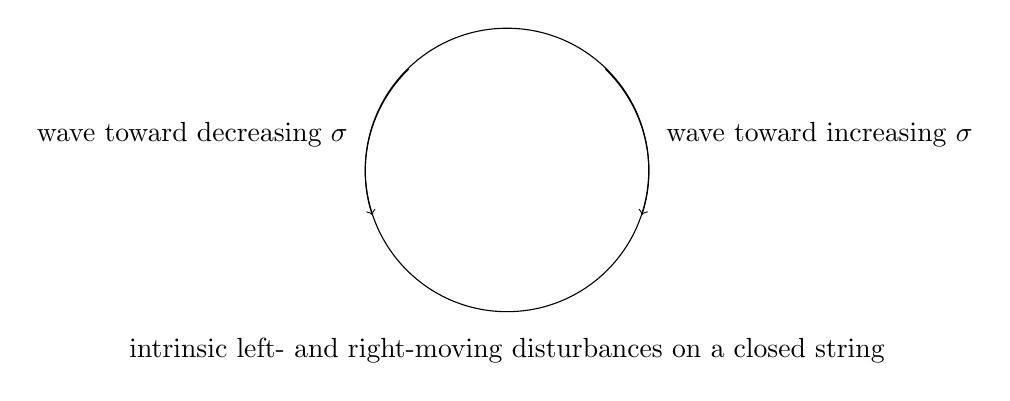
\begin{tikzpicture}[scale=1.0]
\draw (0,0) circle (1.8);
\draw[->] (1.25,1.28) arc[start angle=46,end angle=-18,radius=1.8];
\draw[->] (-1.25,1.28) arc[start angle=134,end angle=198,radius=1.8];
\node[right] at (1.9,0.45) {wave toward increasing \(\sigma\)};
\node[left] at (-1.9,0.45) {wave toward decreasing \(\sigma\)};
\node at (0,-2.3) {intrinsic left- and right-moving disturbances on a closed string};
\end{tikzpicture}
\caption{A cleaned companion picture of the two running-wave sectors.}
\end{figure}

Once the Fourier expansion is plugged into the Lagrangian, each mode amplitude becomes a harmonic oscillator. The key difference from the open string is that each frequency now comes in two directional copies. The closed string therefore has twice as many oscillator families.

Here the notation becomes a little ugly, and Susskind says so himself. We keep his notation, but cleanly. In the \(x\)-sector the creation operators are
\begin{equation}
a_n^+,\qquad a_{-n}^+,
\end{equation}
and in the \(y\)-sector they are
\begin{equation}
b_n^+,\qquad b_{-n}^+.
\end{equation}
The superscript \(+\) means ``creation operator.'' The sign of the subscript records the propagation direction. The symbol \(a\) versus \(b\) tells us whether the excitation is in the \(x\)-direction or the \(y\)-direction. This bookkeeping is clumsy, but it is the bookkeeping of the lecture, and it encodes the essential point: a closed string has a doubled oscillator structure because it supports both left-moving and right-moving running waves.

\section{The First Spectrum Puzzle and the Level-Matching Rule}

The lecture now pivots by recap. Before trying to understand the closed-string spectrum, Susskind reminds us what happened for the open string. There the lowest nontrivial excitations were created by
\begin{equation}
a_1^+|0\rangle,
\qquad
b_1^+|0\rangle,
\end{equation}
and the circular combinations
\begin{equation}
\big(a_1^+\pm i b_1^+\big)|0\rangle
\end{equation}
carried angular momentum \(\pm1\) about the direction of motion. That was the photon story.

If we imitate this too quickly for the closed string, the first states we would write down are
\begin{equation}
a_1^+|0\rangle,\qquad
a_{-1}^+|0\rangle,\qquad
b_1^+|0\rangle,\qquad
b_{-1}^+|0\rangle.
\end{equation}
At first glance this looks perfectly reasonable. It seems to say that we now have two copies of the old photon-like excitation, one associated with one direction of motion along the string and one associated with the other. Susskind even pushes the naïve picture far enough to note that these would have to behave like massless particles, because there is no angular-momentum-zero partner among them.

And then he abruptly says: this is not the right picture.

He makes the tension sharper by looking one level higher. If one simply keeps writing down all states of the next energy, one gets a mess: too many states, the wrong combinations, and no sensible organization into rotational multiplets. That is the point at which he tells us that not every oscillator expression we can write corresponds to a legitimate state of the closed string.

\subsection{Question \& Answer}

\paragraph{Question.} Why is the naïve doubled-photon picture not the right closed-string spectrum?

\paragraph{Answer.} Because the closed string comes with a constraint. One does \emph{not} keep every state that can be written down from the oscillators. The rule, given first as a postulate and only later derived, is the level-matching condition:
\begin{equation}
E_L=E_R.
\end{equation}
The total left-moving energy must equal the total right-moving energy.

That single rule immediately kills the four one-oscillator states above. Each of them carries energy only in one running-wave sector. The same thing happens to the obvious energy-two states
\begin{equation}
a_2^+|0\rangle,\qquad
a_{-2}^+|0\rangle,\qquad
b_2^+|0\rangle,\qquad
b_{-2}^+|0\rangle,
\end{equation}
because these too carry two units of energy in only one direction. In the lecture Susskind quite literally crosses such states out. The rule is presented first as an unexplained but necessary restriction, and only later are we told why it is true.

\section{Massless Spin-2, Dilaton, and Axion}

Once level matching is imposed, the first nontrivial surviving states appear at total excitation energy two:
\begin{equation}
a_1^+a_{-1}^+|0\rangle,\qquad
b_1^+b_{-1}^+|0\rangle,\qquad
a_1^+b_{-1}^+|0\rangle,\qquad
a_{-1}^+b_1^+|0\rangle.
\end{equation}
Each one carries one unit of right-moving energy and one unit of left-moving energy. These are therefore legitimate states.

Now we rewrite them in the circular-polarization basis. The four independent combinations may be taken to be
\begin{align}
\big(a_1^+ + i b_1^+\big)\big(a_{-1}^+ + i b_{-1}^+\big)|0\rangle,\label{eq:spin2plus}\\
\big(a_1^+ - i b_1^+\big)\big(a_{-1}^+ - i b_{-1}^+\big)|0\rangle,\label{eq:spin2minus}\\
\big(a_1^+ + i b_1^+\big)\big(a_{-1}^+ - i b_{-1}^+\big)|0\rangle,\label{eq:scalarone}\\
\big(a_1^+ - i b_1^+\big)\big(a_{-1}^+ + i b_{-1}^+\big)|0\rangle.\label{eq:scalartwo}
\end{align}
The corresponding angular momenta about the axis of motion are
\begin{equation}
M=+2,\qquad -2,\qquad 0,\qquad 0.
\end{equation}

A compact way to display the bookkeeping is the following.

\begin{table}[t]
\centering
\begin{tabular}{c c}
state & angular momentum \(M\) \\
\(\big(a_1^+ + i b_1^+\big)\big(a_{-1}^+ + i b_{-1}^+\big)|0\rangle\) & \(+2\) \\
\(\big(a_1^+ - i b_1^+\big)\big(a_{-1}^+ - i b_{-1}^+\big)|0\rangle\) & \(-2\) \\
\(\big(a_1^+ + i b_1^+\big)\big(a_{-1}^+ - i b_{-1}^+\big)|0\rangle\) & \(0\) \\
\(\big(a_1^+ - i b_1^+\big)\big(a_{-1}^+ + i b_{-1}^+\big)|0\rangle\) & \(0\)
\end{tabular}
\caption{Lowest level-matched closed-string states in the circular basis.}
\end{table}

The crucial interpretation now comes exactly in the rhythm of the lecture. First: we have states with \(M=\pm2\). Could this be a spin-two particle? A \emph{massive} spin-two particle would have five states, with \(M=2,1,0,-1,-2\). Those are not here. We are missing the \(M=\pm1\) pieces entirely. Therefore the only sensible reading is that the \(M=\pm2\) pair is a \emph{massless} spin-two particle. In other words, the closed string contains the graviton.

Then comes the second step: what is left over? The answer is two independent \(M=0\) states. The lecture identifies these as two scalar particles. One linear combination is the dilaton; the other is the axion. Susskind does not derive the normalized combinations carefully on the board, so we should not pretend to do more than the lecture does. The safe statement is that the lowest level-matched closed-string sector contains
\begin{equation}
\text{graviton} \;+\; \text{dilaton} \;+\; \text{axion},
\end{equation}
all massless at this stage of the formal discussion.

This is the first real payoff of the closed-string spectrum. Open strings gave the photon. Closed strings, once the extra constraint is imposed, give the graviton.

\section{Why Level Matching Holds: Shifting the Origin of \(\sigma\)}

Only one major question is left hanging: why should the left-moving and right-moving energies be equal? Here the lecture returns to the marked point \(\sigma=0\) and asks whether it was ever physical to begin with.

A good place to start is the discrete string. Think of the loop as a large collection of points. Then instead of \(X(\sigma)\) and \(Y(\sigma)\), one writes
\begin{equation}
X(\sigma),\qquad X_i,\qquad Y_i,\qquad i=1,\ldots,N.
\end{equation}
The board layout for this step is worth keeping because it shows the discrete loop, the notation, and the wavefunction block together:

\begin{figure}[t]
\centering

\includegraphics[width=0.82\textwidth]{lecture_04_figure_03.png}
\caption{Discrete closed string and cyclic wavefunction labeling.}
\end{figure}

A clean schematic of the discretized loop is useful nearby:

\begin{figure}[t]
\centering
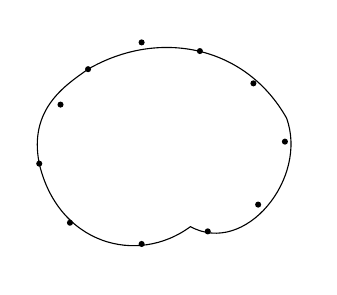
\begin{tikzpicture}[scale=1.0]
\draw
(0.2,1.0)
.. controls (1.1,1.52) and (2.2,1.3) .. (2.72,0.38)
.. controls (3.0,-0.38) and (2.2,-1.38) .. (1.5,-1.0)
.. controls (0.82,-1.5) and (-0.18,-1.22) .. (-0.42,-0.2)
.. controls (-0.56,0.5) and (-0.08,0.8) .. (0.2,1.0);
\foreach \p in {(0.2,1.0),(0.88,1.34),(1.62,1.23),(2.3,0.82),(2.7,0.08),(2.36,-0.72),(1.72,-1.06),(0.88,-1.22),(-0.03,-0.95),(-0.42,-0.2),(-0.15,0.55)}
{\fill \p circle (1.1pt);}
\end{tikzpicture}
\caption{A discretized closed loop, used to make cyclic relabeling explicit.}
\end{figure}

To keep the notation from becoming unbearable, the lecture temporarily suppresses the \(Y_i\) variables and speaks only about the \(x\)-coordinates. The quantum state is then a wavefunction
\begin{equation}
\Psi(x_1,x_2,\ldots,x_N).
\end{equation}
But if the point called \(\sigma=0\) is not special, why should the description begin with \(x_1\) rather than \(x_2\)? The natural requirement is not full symmetry under arbitrary reorderings, which would rip the string open, but invariance under cyclic relabeling:
\begin{equation}
\Psi(x_1,x_2,\ldots,x_N)
=
\Psi(x_2,\ldots,x_N,x_1)
=
\Psi(x_3,\ldots,x_N,x_1,x_2).
\end{equation}
In discrete notation the shift is simply
\begin{equation}
X_i \to X_{i+1}.
\end{equation}
This is the real content of ``there is no preferred point on the string.''

Now pass to the continuum. The discrete cyclic shift becomes
\begin{equation}
\sigma \to \sigma+\epsilon.
\end{equation}
The wavefunction is now a functional of the whole profile \(X(\sigma)\). In cleaned form, the board statement is
\begin{equation}
0=\Psi\bigl(X(\sigma+\epsilon)\bigr)-\Psi\bigl(X(\sigma)\bigr),
\end{equation}
with the understanding that the upper line in the blackboard image is cropped and this subtraction is reconstructed from the surrounding transcript. The lecture then zooms in on the first-order variation, and that local structure is visible in the board close-up:

\begin{figure}[t]
\centering

\includegraphics[width=0.70\textwidth]{lecture_04_figure_04.png}
\caption{Small-\(\epsilon\) shift of the wavefunctional argument.}
\end{figure}

At the board level the infinitesimal change is written as
\begin{equation}
\delta\Psi
\sim
\frac{\partial\Psi}{\partial X(\sigma)}
\frac{\partial X}{\partial \sigma}\,\epsilon.
\end{equation}
This is faithful to what is written, but we must immediately say what the lecture itself then says: this is not a separate equation for one special value of \(\sigma\). The shift moves \emph{every} point on the string.

\subsection{Question \& Answer}

\paragraph{Question.} Is \(\sigma=0\) really a physically special point, and is the variation equation separate for each \(\sigma\)?

\paragraph{Answer.} No on both counts. If no point on the loop is physically preferred, then shifting the origin of \(\sigma\) must leave the state unchanged. And since the shift changes the coordinate of every point on the string, one must add the variations from all \(\sigma\)-points. In the continuum that means integrating:
\begin{equation}
\int d\sigma\,
\frac{\delta\Psi}{\delta X(\sigma)}\,\partial_\sigma X(\sigma)=0.
\end{equation}
Here we have upgraded the board's ordinary derivative notation to the appropriate functional derivative notation, but the logic is exactly the lecture's logic.

Now we return to elementary quantum mechanics. Differentiation of the wavefunction with respect to a coordinate is the action of the corresponding momentum operator. Suppressing \(\hbar\),
\begin{equation}
P(\sigma)\sim -\,i\,\frac{\delta}{\delta X(\sigma)}.
\end{equation}
Therefore the invariance condition becomes
\begin{equation}
\int d\sigma\,P(\sigma)\,\partial_\sigma X(\sigma)=0.
\end{equation}
The board transition into this formula is partly preserved in the next frame:

\begin{figure}[t]
\centering

\includegraphics[width=0.72\textwidth]{lecture_04_figure_05.png}
\caption{Discrete shift and the emerging reparameterization constraint.}
\end{figure}

In the simple nonrelativistic string model used throughout these lectures, momentum is just velocity, so
\begin{equation}
P(\sigma)=\partial_\tau X(\sigma).
\end{equation}
Hence the constraint becomes
\begin{equation}
\int d\sigma\,\partial_\tau X\,\partial_\sigma X=0.
\end{equation}
This is already the essential result. To see why it is level matching, compare it with the left-right decomposition of the energy. Suppressing the duplicated transverse directions for a moment, the difference of the two energy densities is
\begin{equation}
\frac12
\Big[
(\partial_\tau X+\partial_\sigma X)^2
-
(\partial_\tau X-\partial_\sigma X)^2
\Big]
=
2\,\partial_\tau X\,\partial_\sigma X.
\end{equation}
So, up to the same harmless normalization ambiguity that Susskind himself flags on the board,
\begin{equation}
E_L-E_R \propto \int d\sigma\,\partial_\tau X\,\partial_\sigma X.
\end{equation}
But the integral on the right must vanish if the theory is invariant under shifting the origin of \(\sigma\). Therefore
\begin{equation}
E_L=E_R.
\end{equation}

This is the beautiful fact the lecture is aiming at. Level matching is not an arbitrary cleanup rule imposed after the fact. It is the statement that the closed string has no physically distinguished point. And the rule throws away exactly the large chunk of the naïve spectrum that refused to organize itself into sensible particle multiplets.

\section{Clarifications, Fundamentality, and the M-Theory Turn}

The lecture closes by cleaning up one possible confusion and then widening the horizon.

The confusion is linguistic. Susskind has used the words ``left'' and ``right'' in two different senses. One sense refers to intrinsic propagation along the string: motion toward increasing \(\sigma\) or decreasing \(\sigma\). The other sense refers to circular polarization in ordinary \(x\)-\(y\) space, as when one speaks of right-handed or left-handed photon polarization. These are completely different notions. The first has to do with the sign of \(n\); the second has to do with combinations like \(a\pm i b\). The lecture returns to this point explicitly, and the notes should do the same.

Then comes the philosophical coda. After all the formal machinery of open and closed strings, one may ask whether strings are truly fundamental. Susskind answers this by backing away from the word itself. The better question is not which object is ultimately fundamental in some absolute metaphysical sense, but which description is useful in a given regime of parameters. He illustrates the point with electric charges and magnetic monopoles: in one range of coupling constants the electric variables are simple and the magnetic variables are heavy and complicated; in another range the roles can reverse. The same moral carries over to string theory. There are regimes in which it is useful to think of strings as the fundamental objects, and other regimes in which D-branes become the simpler degrees of freedom and strings look more composite.

That is the lesson the lecture wants to leave us with before the next turn. Physics does not seem to be marching toward one final smallest ingredient in any naïve reductionist sense. Rather, the useful elementary objects can change as the parameters of the theory change. The next subject will be M-theory, where exactly that kind of change of viewpoint becomes indispensable.

\subsection{Summary}

The lecture begins with Noether's theorem because a symmetry argument is waiting in the wings. We then draw a closed string, mark a point \(\sigma=0\), and insist that the mark is only conventional. Periodicity leads to Fourier modes with positive and negative integers, and the closed-string energy naturally splits into left-moving and right-moving pieces. That split doubles the oscillator structure.

A naïve first look at the spectrum suggests a doubled photon story, but the lecture deliberately interrupts that guess. The correct rule is level matching: left-moving and right-moving energies must be equal. Once that rule is imposed, the first surviving closed-string excitations assemble into a massless spin-two particle together with two scalar states. The graviton appears, and beside it the dilaton and axion.

Finally, the deferred explanation is supplied. Level matching follows from invariance under shifting the origin of the \(\sigma\)-coordinate. A closed string with no preferred point on the loop must satisfy a momentum constraint, and that constraint is precisely the vanishing of the difference between left-moving and right-moving energies. In this way the geometry of the closed loop, the symmetry of its parameterization, and the structure of the spectrum all lock together.